           %%%%%%%%%%%%%%%%%%%%%%%%%%%%%%%%%%%%
           %    Autore: Giuseppe Silano       %
           %%%%%%%%%%%%%%%%%%%%%%%%%%%%%%%%%%%%

   %%%%%%%%%%%%%%%%%%%%%%%%%%%%%%%%%%%%%%%%%%%%%%%%%%
   %%%%%  Ultima modifica:  14 Febbraio 2020    %%%%%
   %%%%%%%%%%%%%%%%%%%%%%%%%%%%%%%%%%%%%%%%%%%%%%%%%%



                                 %            %%
                                 %             %
   %%%%  % %%   %%%   %%%% %%%%  %%%%   %%%    %    %%%
   %   % %%  % %   % %   % % % % %   % %   %   %   %   %
   %   % %     %%%%% %   % % % % %   % %   %   %   %   %
   %   % %     %     %  %% % % % %   % %   %   %   %   %
   %%%%  %      %%%%  %% % % % % %%%%   %%%   %%%   %%%
   %
   %
   
% CHANGELOG
% 14 Febbraio 2020: Aggiornato Logo UniSannio
% 11 Luglio 2018: Prima versione


%Le parole italian ed english istruiscono il tex a sillabare una porzione di testo con le regole rispettivamente in italiano ed inglese. Per passare da italiano ad inglese è sufficiente utilizzare il comando \selectlanguage{english}, per tornare poi all'italiano \selectlanguage{italian}
\documentclass[11pt,a4paper,oneside,english,italian]{book} 

% Usare "oneside" invece di "twoside" nelle bozze, per risparmiare carta: "twoside" produce diverse pagine bianche alla fine dei capitoli.

%Questo pacchetto consente di impostare i margini del documento. La prola headsep sta indicare l'altezza dell'intestazione, mentre il footskip indica la dimensione dello scalino a piè pagina
\usepackage[a4paper]{geometry}
\geometry{verbose, tmargin=4cm, bmargin=4cm, lmargin=3cm, rmargin=3cm, headsep=0.5cm, footskip=1cm}

%Necessario per creare delle box in un'immagine
\usepackage[export]{adjustbox}

%Necessario per inserire pdf in latex
\usepackage[final]{pdfpages}

%Per poter esportare i grafici da Matlab
\usepackage{pgfplots}

                    %%%%%%%%%%%%%%%%%%%%%%%%%%%%%%%%
                    %         inputenc             %
                    %  Usare l'opzione "latin1"    %
                    %  se si vogliono scrivere     %
                    %  lettere accentate da        %
                    %  tastiera su Windows o Unix  %
                    %%%%%%%%%%%%%%%%%%%%%%%%%%%%%%%%

%\usepackage[latin1]{inputenc}
\usepackage[utf8x]{inputenc}		%Nel caso questo file tex venga compilato in ambiente Linux

			 %%%%%%%%%%%%%%%%%%%%%%%%%%%%%%%%%%%%%%%%%%%%%%%
			 %                  mcode                      %
			 % Consente l'inserimento di codice Matlab nel %
			 % fil tex									   %
			 %%%%%%%%%%%%%%%%%%%%%%%%%%%%%%%%%%%%%%%%%%%%%%%

%Il file mcode.sty è presente nella stessa cartella del codice .tex
%Si tratta di una valida alternativa a lstlisting se si vuole inserire del codice all'interno della presentazione
\usepackage[framed,numbered,autolinebreaks,useliterate]{mcode}
   
%Per ruotare le pagine in LaTeX: consente di ruotare la pagina in senso orario di 90°
\usepackage{pdflscape}

%Package necessario per disegnare in LaTeX. A seconda del disegno che si realizza è necessario
%importare delle librerie piuttosto che altre.
\usepackage{tikz}

       %%%%%%%%%%%%%%%%%%%%%%%%%%%%%%%%%%%%%%%%%%%%%%
       %                  babel                     %
       %    Pacchetto tipico per la stesura di un   %
       %    dcoumento in italiano.                  %
       %%%%%%%%%%%%%%%%%%%%%%%%%%%%%%%%%%%%%%%%%%%%%%

\usepackage[italian]{babel}

%Pacchetto necessario ad impostare l'interlinea
\usepackage{setspace}

%Package impiegato per editare e formattare opportunamente frammenti di pseudocodice.
\usepackage{algorithmic}

%algorithm serve per incapsulare algorithmic al fine di ottenere un oggetto flotable come una figura o una tabella.
\usepackage{algorithm} 
%\usepackage{algpseudocode}

%Package per inserire "facilmente" le unità di misura del sistema metrico internazionale
\usepackage{siunitx} 

%Inserire pseudoalgoritmo in italiano
\makeatletter
\newcommand{\newalgname}[1]{
	\renewcommand{\ALG@name}{#1}
}
\newalgname{Algoritmo} %Tutti gli algoritmi saranno chiamati "Algoritmo"
\renewcommand{\listalgorithmname}{Lista dei \ALG@name s} %Stesso discorso affrontato in precedenza
\makeatother

%Il pacchetto tocbibind fa comparire nell'indice la bibliografia ed eventualmente l'indice analitico
\usepackage[nottoc]{tocbibind}

% Pacchetto graphicx per inserire figure in LaTeX. Maggiori dettagli sull'utilizzo del pacchetto sono riportati di seguito.
\usepackage{graphicx} 
\graphicspath{{./figure/}}
\usepackage{epstopdf}
%\usepackage{subfigure}
\newcommand{\goodgap}{
	\hspace{\subfigtopskip}
	\hspace{\subfigbottomskip}}

%%%%%%%%%%%%%%%%%%%%%%%%%%%%%%%%%%%%%%%%%%%%%%%%%%%%%%%
%                    graphicx                         %
%                                                     %
%   Uno dei pacchetti per l'inserzione di figure      %
%   in formato eps e` "graphicx". Ce ne sono diversi  %
%   altri da poter scegliere.                         %
%                                                     %
%   Esempio di uso: avendo un file di nome            %
%   figura1.eps questa si inserisce nella tesi        %
%   col comando                                       %
%                                                     %
%        \begin{figure}[ht]                           %
%        \begin{center}                               %
%        \includegraphics{figura1.eps}                %
%        \caption[nome breve]{nome lungo}             %
%        \label{etichetta}                            %
%        \end{center}                                 %
%        \end{figure}                                 %
%                                                     %
%   Il "nome breve" e` quello che apparira`           %
%   nell'indice delle figure ed e' opzionale.         %
%   Il "nome lungo" e' quello che appare              %
%   sotto la figura.                                  %
%   (Ci sono opzioni per scalare, spostare, ruotare   %
%   le figure).                                       %
%   Con \graphicspath{{./figure/}} si dice            %
%   al LaTeX di cercare le figure nella cartella      %
%   "figure" situata allo stesso livello di           %
%   questo documento                                  %
%                                                     %
%%%%%%%%%%%%%%%%%%%%%%%%%%%%%%%%%%%%%%%%%%%%%%%%%%%%%%%


%Questi pacchetti consentono di centrare il contenuto di una tabella
\usepackage{multirow}
\usepackage{comment}
\usepackage{array}
\newcolumntype{P}[1]{>{\centering\arraybackslash}p{#1}}
\newcolumntype{M}[1]{>{\centering\arraybackslash}m{#1}}
\newcolumntype{L}[1]{>{\arraybackslash}m{#1}}
\usepackage{xcolor,colortbl}
\usepackage{tabularray}
\definecolor{red}{rgb}{1,0,0}

  %%%%%%%%%%%%%%%%%%%%%%%%%%%%%%%%%%%%%%%%%%%%%%%%%%%%%%%%%%%%%%%%%%%%%%%%%%%%%%%%%%%%%%%%%%%%%%%%%%%%%%%%%%%%%%%%%%%%%%%%%%%%%%%%%%%%%%%%%%%
  % Dettagli del documento. Non compaiono direttamente nel documento ma sono conservate al suo interno. Tali informazioni sono accessibili  %
  % utilizzando la funzione "File>Document Properites>Description". Utili per scopi archivistici											%
  %%%%%%%%%%%%%%%%%%%%%%%%%%%%%%%%%%%%%%%%%%%%%%%%%%%%%%%%%%%%%%%%%%%%%%%%%%%%%%%%%%%%%%%%%%%%%%%%%%%%%%%%%%%%%%%%%%%%%%%%%%%%%%%%%%%%%%%%%%%

\usepackage{hyperref}  
\hypersetup{
	% pdfpagelayout=SinglePage, % default
	% pdfpagemode=UseOutlines, % default
	% bookmarksopen, % default
	% bookmarksopenlevel=2, % default;
	%pdftitle={Modello non ufficiale tesi di laurea all'Università degli Studi del Sannio in Benevento},
	%pdfauthor={Giuseppe Silano},
	%pdfsubject={Lo scopo di questo template è quello di favorire gli studenti, di UniSannio e non, nella scrittura della propria tesi di laurea in LaTeX},
	%pdfkeywords={UniSannio, tesi, template, LaTeX}} 
    pdftitle={Progetto di Sistemi Cyberfisici di Mattia Marino},
    pdfauthor={Mattia Marino}
}

%%%%%%%%%%%%%%%%%%%%%%%%%%%%%%%%%%%%%%%%%%%%%%%%%%%%%%%%%%%%

       %%%%%%%%%%%%%%%%%%%%%%%%%%%%%%%%%%%%%%%%%%%%%%%%
       % Pacchetti tipici per un report di Ingegneria %
       %%%%%%%%%%%%%%%%%%%%%%%%%%%%%%%%%%%%%%%%%%%%%%%%

\usepackage{amsmath, amsfonts, amssymb, amsthm}
\usepackage{latexsym}
\usepackage{lmodern}
\usepackage[T1]{fontenc}

   %%%%%%%%%%%%%%%%%%%%%%%%%%%%%%%%%%%%%%%%%%%
   %  Esempi di macro definite dall'utente.  %
   %  Le prime definiscono dei comandi per   %
   %  scrivere i caratteri speciali per      %
   %  gli insiemi numerici fondamentali      %
   %  (naturali, interi, razionali, reali,   %
   %  complessi                              %
   %%%%%%%%%%%%%%%%%%%%%%%%%%%%%%%%%%%%%%%%%%%

\newcommand{\N}{\mathbb{N}}
\newcommand{\Z}{\mathbb{Z}}
\newcommand{\Q}{\mathbb{Q}}
\newcommand{\R}{\mathbb{R}}
\newcommand{\C}{\mathbb{C}}

   %%%%%%%%%%%%%%%%%%%%%%%%%%%%%%%%%%%%%%%%%%%%
   %  Delle macro che definiscono operatori   %
   %  non predefiniti in LaTeX. Ogni utente   %
   %  aggiunge quelle che servono. Questi     %
   %  sono solo esempi arbitrari.             %
   %%%%%%%%%%%%%%%%%%%%%%%%%%%%%%%%%%%%%%%%%%%%

\DeclareMathOperator{\traccia}{tr}
\DeclareMathOperator{\sen}{sen}
\DeclareMathOperator{\arcsen}{arcsen}
\DeclareMathOperator*{\maxlim}{max\,lim}
\DeclareMathOperator*{\minlim}{min\,lim}
\DeclareMathOperator*{\deepinf}{\phantom{\makebox[0pt]{p}}inf}
\DeclareMathOperator*{\argmin}{argmin}

    %%%%%%%%%%%%%%%%%%%%%%%%%%%%%%%%%%%%%%%%%%%%
    % Esempi di macro piu` elaborate,          %
    % contenenti degli argomenti.              %
    % Compongono gli indici delle sommatorie   %
    % e delle produttorie in modo diverso      %
    % da quello standard del TeX. Dovrebbero   %
    % funzionare bene quando gli estremi della %
    % sommatoria sono piccoli. 			       %
    %%%%%%%%%%%%%%%%%%%%%%%%%%%%%%%%%%%%%%%%%%%%

\newcommand{\varsum}[3]{\sum_{#2}^{#3}\!
   {\vphantom{\sum}}_{#1}\;}
\newcommand{\varprod}[3]{\sum_{#2}^{#3}\!
   {\vphantom{\sum}}_{#1}\;}

  %%%%%%%%%%%%%%%%%%%%%%%%%%%%%%%%%%%%%%%%%%%%%%%%%%%%%%%
  %          Numerazione delle formule                  %
  % Se non specificato altrimenti, il LaTeX numera le   %
  % formule come (capitolo.formula) (per esempio (2.5)  %
  % e` la quinta formula del secondo capitolo).         %
  % Con le istruzioni seguenti invece la numerazione    %
  % diventa (capitolo.sezione.formula) (per esempio     %
  % (3.2.6) e` la sesta formula della seconda sezione   %
  % del terzo capitolo):                                %
  %%%%%%%%%%%%%%%%%%%%%%%%%%%%%%%%%%%%%%%%%%%%%%%%%%%%%%%

%\makeatletter
%\@addtoreset{equation}{section}
%\makeatother
%\renewcommand{\theequation}%
%  {\thesection.\arabic{equation}}


              %%%%%%%%%%%%%%%%%%%%%%%%%%
              % Stile degli enunciati  %
              %%%%%%%%%%%%%%%%%%%%%%%%%%

%%%%%%%%%%%%%%%%%%%%%%%%%%%%%%%%%%%%%%%%%%%%%%%%%%%%%%%%%%%
% Con le dichiarazioni seguenti                           %
% teoremi, definizioni, proposizioni, lemmi e corollari   %
% vengono numerati capitolo per capitolo e con un         %
% contatore unico per tutti (per esempio, se subito dopo  %
% il Teorema 2.1 c'e' una definizione, questa sara'       %
% Definizione 2.2)                                        %
%%%%%%%%%%%%%%%%%%%%%%%%%%%%%%%%%%%%%%%%%%%%%%%%%%%%%%%%%%%

\theoremstyle{plain}
\newtheorem{teorema}{Teorema}[chapter]
\newtheorem{proposizione}[teorema]{Proposizione}
\newtheorem{lemma}[teorema]{Lemma}
\newtheorem{corollario}[teorema]{Corollario}

\theoremstyle{definition}
\newtheorem{definizione}[teorema]{Definizione}
\newtheorem{esempio}[teorema]{Esempio}

\theoremstyle{remark}
\newtheorem{osservazione}[teorema]{Osservazione}

  %%%%%%%%%%%%%%%%%%%%%%%%%%%%%%%%%%%%%%%%%%%%%%%%%%%%%%%%
  % I comandi si usano cosi`:                            %
  %                                                      %
  %   \begin{teorema}[di Pitagora]                       %
  %   La somma dei quadrati ecc.                         %
  %   \end{teorema}                                      %
  %                                                      %
  % Le parole "di Pitagora" fra parentesi quadre         %
  % sono facoltative. Non bisogna inserire               %
  % manualmente degli spazi prima e dopo gli enunciati,  %
  % perche' e` automatico!                               %
  %%%%%%%%%%%%%%%%%%%%%%%%%%%%%%%%%%%%%%%%%%%%%%%%%%%%%%%%


  %%%%%%%%%%%%%%%%%%%%%%%%%%%%%%%%%%%%%%%%%%%%%%%%%%%%%%%%%%%%%%
  % Il pacchetto amsthm definisce anche l'ambiente "proof"     %
  % per le dimostrazioni.                                      %
  % Esempio di uso:                                            %
  %                                                            %
  %   \begin{proof}                                            %
  %   Sia $X$ un insieme ecc.                                  %
  %   \end{proof}                                              %
  %                                                            %
  %%%%%%%%%%%%%%%%%%%%%%%%%%%%%%%%%%%%%%%%%%%%%%%%%%%%%%%%%%%%%%

       %%%%%%%%%%%%%%%%%%%%%%%%%%%%%%%%%%%%%%%%%%%%%%%%%%%%%%%
       %                   makeidx                           %
       %                                                     %
       % Pacchetto per la generazione automatica dell'indice %
       % analitico. Per esempio, se vogliamo che la parola   %
       % "analitico" venga indicizzata nella frase           %
       %                                                     %
       %    "un metodo analitico di soluzione"               %
       %                                                     %
       % bisogna scrivere                                    %
       %                                                     %
       %    "un metodo analitico\index{analitico} di         %
       %              soluzione".                            %
       %                                                     %
       % Compilando il file, il LaTeX produrra' un file      %
       % ausiliario che termina con ".idx". Bisogna far      %
       % processare questo file idx dal programma            %
       % ausiliario "bibtex", che produrra' a sua volta un   %
       % altro file ancora. Dare infine un'ultima passata    %
       % col LaTeX. Si puo' tranquillamente lasciare         %
       % la compilazione dell'indice verso la fine della     %
       % stesura del lavoro, quando tutto e' ormai quasi     %
       % definitivo.                                         %
       %                                                     %
       %%%%%%%%%%%%%%%%%%%%%%%%%%%%%%%%%%%%%%%%%%%%%%%%%%%%%%%

%\usepackage{makeidx}
%\makeindex

%Indentazione automatica anche nel primo paragrafo
\usepackage{indentfirst}

%Per inserire i linguaggi di programmazione
\usepackage{listings}

%Necessario per inserire l'appendice
\usepackage{appendix}
\usepackage[utf8x]{inputenc}
%Redifinizione della riga di testa delle pagine:
\usepackage{fancyhdr}
\pagestyle{fancy}

%Documentazione on-line del package al link: http://www.ctan.org/tex-archive/info/italian/fancyhdr/itfancyhdr.pdf
\usepackage{fancyhdr}
\pagestyle{fancy} %Stile che consente di inserire le barre nei capitoli con il nome dell'attuale sezione ed il numero della pagina
\renewcommand{\chaptermark}[1]{\markboth{#1}{}}
\renewcommand{\sectionmark}[1]{\markright{\thesection\ #1}}
\fancyhf{}
\fancyhead[LE,RO]{\bfseries\thepage}
\fancyhead[LO]{\bfseries\rightmark}
\fancyhead[RE]{\bfseries\leftmark}
\renewcommand{\headrulewidth}{0.5pt}
\renewcommand{\footrulewidth}{0.5pt}
\setlength{\headheight}{14.5pt}

%Pacchetti addizionali per inserire più tabelle o figure fianco a fianco
\usepackage{caption}
\usepackage{subcaption}
\usepackage{booktabs}
\usepackage{float}

               %%%%%%%%%%%%%%%%%%%%%%%%%%%%%%%%%%%%%%
               %          Corpo dell report         %
               %%%%%%%%%%%%%%%%%%%%%%%%%%%%%%%%%%%%%%               
	

%Da qui inizia il documento, fino ad ora si è preparato il preambolo
\begin{document}

%Titolo della tesi
\frontmatter


  %%%%%%%%%%%%%%%%%%%%%%%%%%%%%%%%%%%%%%%%%%%%%%%%%%%%%%%%%%%
  %   Si puo` scegliere fra scrivere tutta la tesi in un    %
  %   solo file, oppure distribuire ogni capitolo in un     %
  %   file a parte. Qui si e` scelto tenere separati i      %
  %   vari capitoli, che vengono caricati con \include      %
  %  questo facilita non solo la fase di revisione ma       %
  %  ma anche la lettura del codice TeX attraverso un ap-   %
  %  -proccio di tipo modulare
  %%%%%%%%%%%%%%%%%%%%%%%%%%%%%%%%%%%%%%%%%%%%%%%%%%%%%%%%%%%

\renewcommand{\theequation}{\arabic{equation}}%consigliato per migliorare i numeri di equazione nell'introduzione
\renewcommand{\thesection}{\arabic{section}}  %consigliato per migliorare i numeri di equazione nell'introduzione

%Frontespizio e dedica della tesi
\linespread{1} % per il frontespizio utilizzo l'interlinea singola

\thispagestyle{empty}
\large

% % % % % % % % % % % % % % % % % % % % 
% TESTO IN CORSIVO
% % \emph{\textbf{UNIVERSITA' DEGLI STUDI DEL SANNIO}}\\
% % \textbf{\emph{Facolt?  di Ingegneria}}\\
% % \textbf{\emph{Corso di Laurea Specialistica in \\Ingegneria delle
		% % Telecomunicazioni}}
% % % % % % % % % % % % % % % % % % 

% INTESTAZIONE DEL FRONTESPIZIO
\begin{center}
	\huge{{\underline{\textsc{UNIVERSIT\`A DEGLI STUDI DEL SANNIO}}}}
\end{center}

\begin{center}   
	\huge{{\textsc{DIPARTIMENTO DI INGEGNERIA}}}
	\\
	\LARGE{\textbf{\\Corso di Laurea Magistrale in \\Ingegneria Informatica}}      
	
\end{center}

%******************************************************************
%                                   Logo Unisannio
%******************************************************************
\begin{figure}[h]
	\begin{center}
		
\includegraphics[scale=0.3]{figure/logo/logoUniSannio_new.jpg}
	\end{center}
\end{figure}
%******************************************************************                                

\vspace{0.25cm}

%
%
% TITOLO DELLA TESI
\begin{center}
    Analisi e Controllo di Sistemi Cyberfisici
    
	{\LARGE \textbf{PROGETTAZIONE DI UN SEMAFORO A CORSIA MULTIPLA ORIENTATO AL PARALLELISMO} \smallskip\\}                                               
\end{center}

% RELATORE E CANDIDATO DELLA TESI
\vspace{2cm}
\begin{tabular}{ll}
	\textit{Prof.ssa:}        \hspace{3cm}   	& \textit{Autore:}\\
	\textbf{Elisa Mostacciuolo}      \hspace{5cm}     & \textbf{Mattia Marino}\\   
	\hspace{3cm}      & \textit{Matr:399000634}                                       					   
	%                        
\end{tabular}

% ANNO ACCADEMICO     
\vspace{2.5cm}
\begin{center}
	\textsc{Anno Accademico 2024/2025}
\end{center}

% Nuova pagina    
\newpage


%Numerazione delle prime pagine in numeri romani
\pagenumbering{roman}

%Set del conunter al valore 1, questo evita che vengono conteggiate anche la pagine del frontespizio, facendo partire il conteggio da 3 piuttosto che da 1
\setcounter{page}{0}

%Indice della tesi
\tableofcontents

%Rispristino il valore dell'interlinea a 1.5, quadunque nel frontespizio venisse posto ad 1.0
\onehalfspacing

%Sommario ed introduzione della tesi che, per come spiegato in precedenza, sono descritti in due
%file tex a parte
%\input{sommario}
\chapter*{Introduzione}
\label{cap:introduzione}

\addcontentsline{toc}{chapter}{Introduzione}
\lhead{\bfseries INTRODUZIONE}
\rhead{\thepage}

Nel contesto tecnologico attuale, i Cyber-Physical Systems (CPS) stanno acquisendo un'importanza sempre maggiore. Questi sistemi integrati, che combinano componenti fisici con capacità computazionali, hanno trasformato vari settori, dall'industria alla sanità, dai trasporti all'energia. Tipicamente, ciò avviene attraverso loop di feedback in cui i processi fisici influenzano la computazione e viceversa. Affinché il sistema possa rispondere ai cambiamenti esterni e correggere il proprio comportamento, è essenziale che la parte fisica e quella computazionale comunichino tramite una rete. I CPS possono impiegare sensori, attuatori, elettronica e software avanzato che collaborano per monitorare, controllare e ottimizzare sistemi reali in tempo reale. Questa interazione tra il mondo cibernetico e quello fisico offre numerosi vantaggi, tra cui maggiore efficienza operativa, sicurezza migliorata, riduzione dei costi e ottimizzazione delle risorse (che nei sistemi embedded sono spesso molto limitate). Questo documento descrive e dettaglia il lavoro svolto nella progettazione e modellazione di un CPS per il controllo di un sistema di semafori stradali in un'intersezione stradale con un focus particolare sul parallelismo dei veicoli che attraversano l'incrocio, qualora possibile.
\chapter*{Problem Statement}
\label{cap:problem-statement}

\addcontentsline{toc}{chapter}{Problem Statement}
\lhead{\bfseries PROBLEM STATEMENT}
\rhead{\thepage}

Il progetto ivi trattato si pone l'obiettivo di progettare e modellare il comportamento di un insieme di semafori stradali in un'intersezione. In particolare, si è scelto di riprogettare un semaforo già esistente, con lo scopo di migliorarne l'efficienza e la sicurezza. Il semaforo scelto a tale scopo è quello presente all'incrocio tra Via del Pomerio, Ponte Vanvitelli, Via Posillipo e Corso Vittorio Emanuele III, a Benevento. Al fine di spiegare meglio la dinamica dell'intersezione, si riportano due schermate catturate da Google Maps, che mostrano l'incrocio in questione (Fig. \ref{fig:intersection_top} e Fig. \ref{fig:intersection_3d}).

\begin{figure}[H]
    \centering
    \begin{minipage}[b]{.45\textwidth}
        \centering
        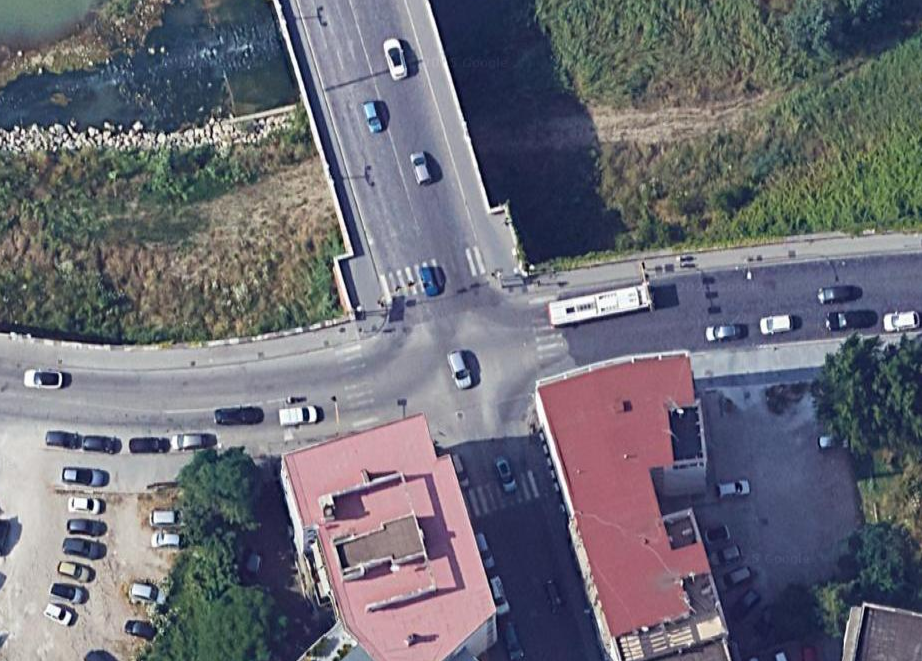
\includegraphics[width=\textwidth]{figure/intersection/incrocio_top.png}
        \caption{Vista dall'alto dell'intersezione}
        \label{fig:intersection_top}
    \end{minipage}
    \hfill
    \begin{minipage}[b]{.45\textwidth}
        \centering
        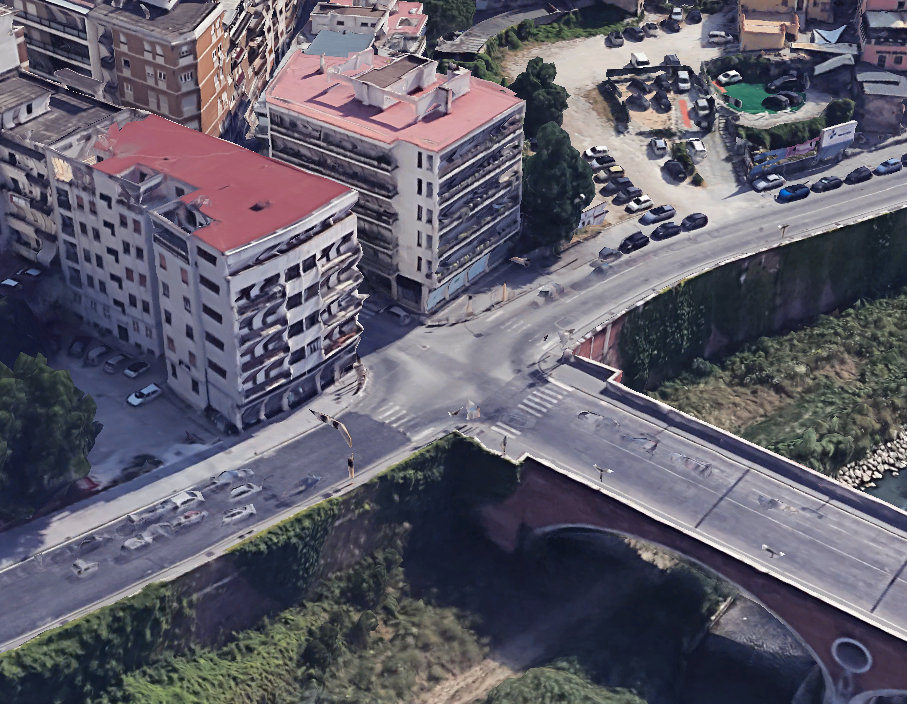
\includegraphics[width=\textwidth]{figure/intersection/incrocio_3d.png}
        \caption{Vista 3D dell'intersezione}
        \label{fig:intersection_3d}
    \end{minipage}
\end{figure}

Come si può quindi dedurre dall'immagine, a Est si trovano tre semafori che consentono di andare a Nord, Sud e Ovest. A Ovest, invece, si trovano due semafori che consentono di andare a Nord e a Sud. Il semaforo a Nord, infine, consente di andare a Ovest o a Sud. Ogni combinazione provenienza-destinazione si trova su un'apposita corsia e ha un semaforo dedicato.

Al fine di modellare il comportamento del semaforo, si è scelto di utilizzare il formalismo delle Reti di Petri, in quanto permette di modellare sistemi concorrenti e distribuiti in modo chiaro e intuitivo. Nel caso modellato, per migliorare l'efficienza del semaforo, si è scelto di permettere il passaggio di più veicoli contemporaneamente, qualora possibile, imponendo vincoli per evitare che due o più veicoli si incrocino. Ad esempio è consentito il passaggio contemporaneo di un veicolo proveniente da Est diretto verso Nord e uno proveniente da Ovest e diretto verso Sud. Al contrario, invece, non è possibile attraversare contemporaneamente l'incrocio con due veicoli provenienti da direzioni diverse e diretti nella stessa direzione, in quanto ciò potrebbe causare un incidente. Inoltre, non è possibile che due veicoli si incontrino all'interno dell'incrocio, come ad esempio un veicolo che attraversa l'incrocio da Est a Ovest e un veicolo che attraversa l'incrocio da Nord a Sud.

Tali vincoli sono stati modellati con l'utilizzo di GMEC, come mostrato nelle sezioni successive.


\renewcommand{\theequation}{\arabic{chapter}.\arabic{equation}} %si torna alle formule numerate come da default
\renewcommand{\thesection}{\arabic{chapter}.\arabic{section}} %consigliato per migliorare i numeri di equazione nell'introduzione

%Da inserirsi prima dei tex in cui vi è il corpo della tesi, i diversi capitoli, pena mancato
%avvio del conteggio
\mainmatter

%Da qui in poi sono riportati i tex contenenti i capitoli della tesi. I diversi capitoli sono
%richiamati all'interno del preambolo utilizzando il comando \include. Inoltre, attraverso il 
%comando \part è possibile suddividere la tesi in parti che prendo il nome dal testo racchiuso tra
%parentesi graffe


%Parte che richiama gli appendici
%\part{Appendici}

%Cambia la numerazione da numeri a lettere
\renewcommand{\thesection}{\Alph{chapter}.\arabic{section}}

%File LaTeX per la gestione degli appendici
%\begin{appendices}
%\input{AppendiceA}
%\end{appendices}

\backmatter

\nocite{*}

%La bibliografia è scritta utilizzando lo stile IEEE Transaction. I contenuti bibliografici, da poi richiamare nel testo, sono descritti nel file .bib
\bibliographystyle{IEEEtran_italiano}

\end{document}